% !TEX root=../root.tex

%\subsection{Related Works}

The Linear Quadratic Regulator (LQR) is a well-known feedback controller that
computes the optimal feedback gains for a linear time-invariant (LTI) system
given a quadratic cost function. LQR has been used to control multirotor UAVs with a variety of
approaches. Almost all of these approaches
linearize the system at a given stable state and use a fixed LQR
gain~\cite{cowling2007prototype}. Some have
used a gain scheduling approach with a library of LQR gains for different
magnitudes of deviation from the desired state~\cite{reyes2013lqr}. Recently, an approach was
proposed that relinearizes the system at a fixed rate, slower than the control
loop, and then recomputes the LQR gains at that rate~\cite{foehn2018onboard}. Our
proposed solution takes a similar approach while relinearizing and recomputing
the LQR gains at every control step. 

Recently there has been a movement in the robotics community to appropriately
deal with the evolution of a robot's state along a manifold using Lie
theory~\cite{sola2018micro}. Though these methods have widely been used in the
field of state estimation~\cite{sola2017quaternion,koch2017relative}, a
% field of state estimation~\cite{sola2017quaternion}~\cite{koch2017relative}, a
few methods have emerged that also apply Lie theory to
control~\cite{yu2015high,lee2010geometric}. We propose a formulation of
% control~\cite{yu2015high}~\cite{lee2010geometric}. We propose a formulation of
the LQR problem that properly deals with the manifold nature of the state,
specifically the attitude component. Most previous LQR solutions
for a multirotor UAV use an Euler angle representation of attitude and treat the
tuple of ZYX Euler angles as if it were a vector space~\cite{cowling2007prototype}, even
though it is not~\cite{diebel2006representing}. While some methods use unit
quaternions or rotation matrices to properly represent atttiude, these are also
not inherently a vector space and extra steps are required to orthonormalize or
otherwise force the attitude to stay on the
manifold~\cite{reyes2013lqr,foehn2018onboard}. The proposed solution is
derived from Lie theory and care is taken to ensure that all vector
manipulations are done with
appropriate vector quantities so that the state remains on the manifold.

% \begin{figure}
  % \centering
  % 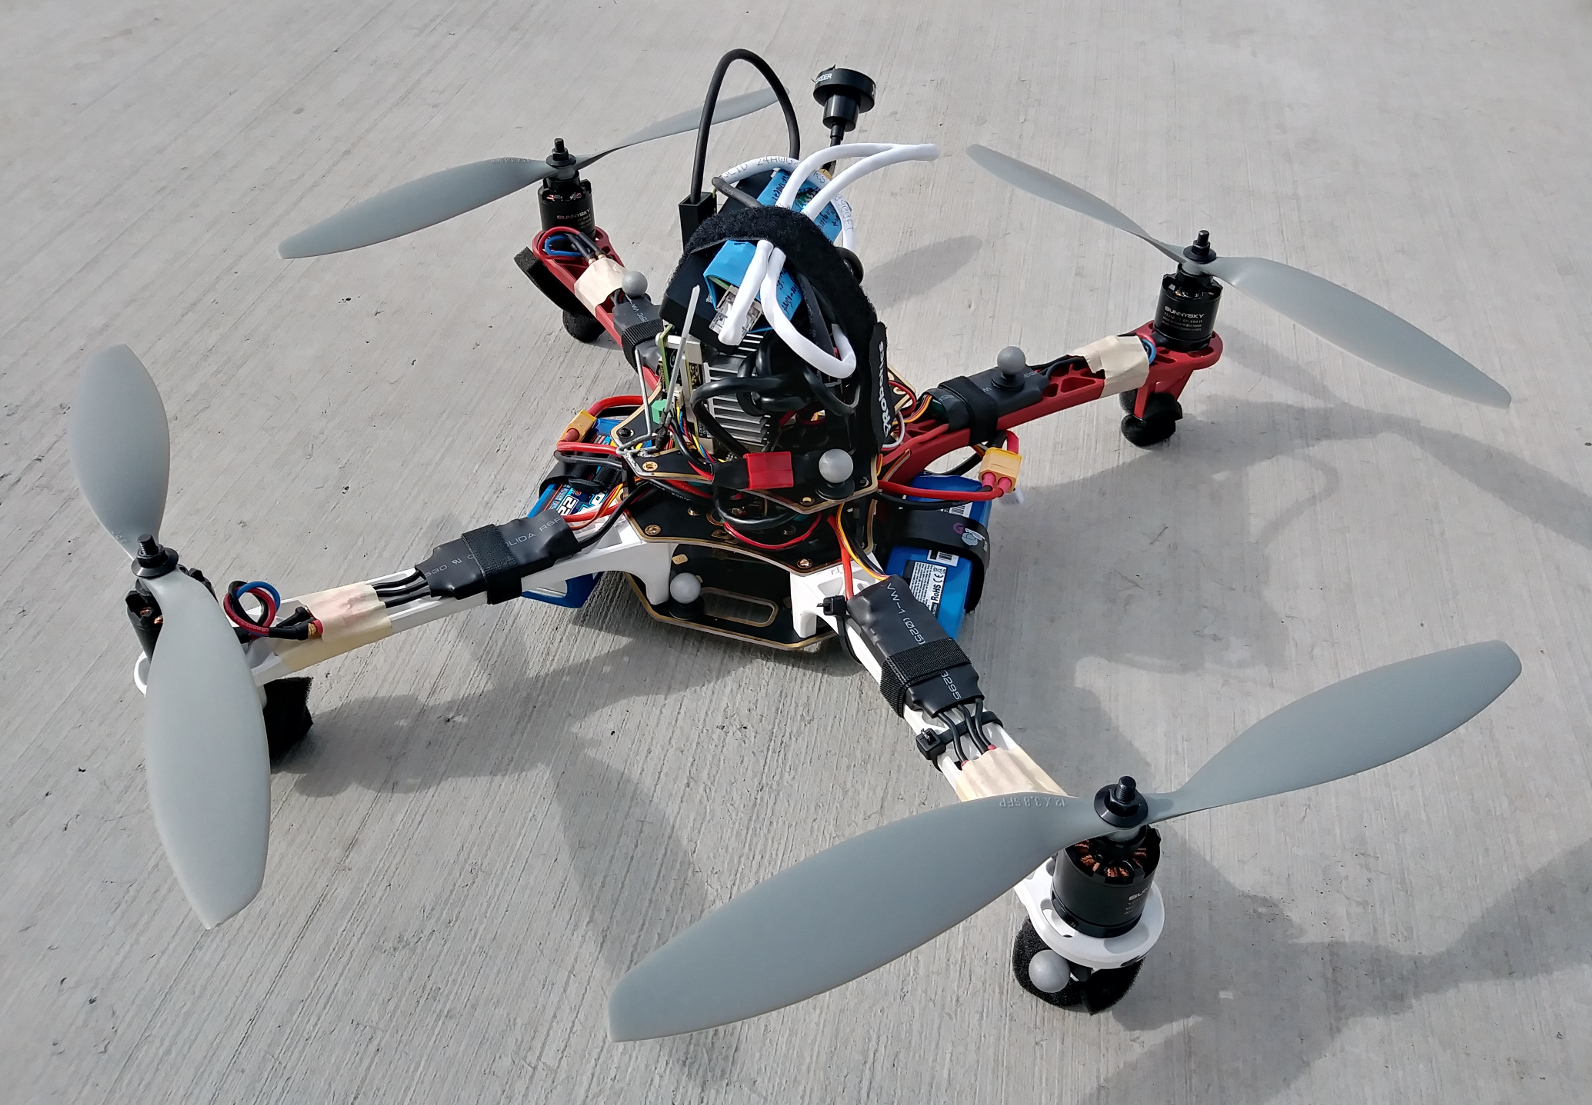
\includegraphics[scale=0.15]{figures/hardware_platform.jpg}
  % \caption[Multirotor UAV Used in Experiments]{Hardware platform used in experiments.}
  % \label{f:drone_pic}
% \end{figure}
